\section{Amogus Trick}

\begin{frame}
\frametitle{Amogus Trick}

\begin{block}{Problem: \href{https://codeforces.com/contest/1594/problem/D}{The Number of Imposters}}
    There are $n$ astronauts in the spacecraft. Each astronaut has to be one of two roles:
    \begin{itemize}
        \item Crewmate
        \item Imposter
    \end{itemize}
    There are $m$ clues from the astronauts (each of which is guaranteed to be true). The clues have only two types:
    \begin{itemize}
        \item $u$ is in the same role as $v$
        \item $u$ is not the same role as $v$
    \end{itemize}
    What is the maximum possible number of imposters?
\end{block}

\end{frame}

\begin{frame}
\frametitle{Amogus Trick}

We can solve this problem with Disjoint Union on $2n$ vertices.

\begin{block}{Definition: Crewmate State}
    parent[1, n] := State of being Crewmate
\end{block}

\begin{block}{Definition: Imposter State}
    parent[n + 1, 2n] := State of being Imposter
\end{block}

\begin{center}
\begin{tabular}{|c||c|c|c|c|c|c|c|c|}
    \hline
    index & 1 & 2 & 3 & 4 & 5 & 6 & 7 & 8\\
    \hline
    \hline
    parent & 1 & 2 & 3 & 4 & 5 & 6 & 7 & 8\\
    \hline
\end{tabular}
\end{center}

\end{frame}

\begin{frame}
\frametitle{Amogus Trick}

Each astronaut $i$ has two vertices:

\begin{itemize}
    \item parent[i]
    \item parent[i + n]
\end{itemize}

\begin{center}
    
\includegraphics[width=4cm]{imgs/amongus_meme.jpg}
\end{center}

\centering
\textit{Credit: Reddit r/AmongUs}

\end{frame}

\begin{frame}
\frametitle{Amogus Trick}

There are two cases:

\begin{enumerate}
    \item $A$ and $B$ share the same role
    \item $A$ and $B$ have different roles
\end{enumerate}

\begin{block}{Case 1: $A$ and $B$ share the same role}
    Unite the two vertices:
    \begin{itemize}
        \item $A$ and $B$
        \item $A + n$ and $B + n$
    \end{itemize}
\end{block}

\begin{block}{Case 2: $A$ and $B$ have different roles}
    Create special edges by unite the two vertices:
    \begin{itemize}
        \item $A$ and $B + n$
        \item $B$ and $A + n$
    \end{itemize}
\end{block}

\end{frame}

\begin{frame}
\frametitle{Amogus Trick}
\textit{Example:}\\
1. $1$ and $2$ are different roles

\begin{center}
\begin{tikzpicture}
[
    edge from parent/.style={thick}
]
    \begin{scope}[edge from parent/.style={draw=blue}]
        \node [draw, circle, blue] {1}
            child {node [draw, circle, blue] {5}};
    \end{scope}
    
    \begin{scope}[edge from parent/.style={draw=red}]
        \node [draw, circle, red] at (3, 0) {2}
            child {node [draw, circle, red] {4}};
    \end{scope}
    
    \begin{scope}[edge from parent/.style={draw=black}]
        \node [draw, circle, black] at (6, 0) {3};
    \end{scope}

    \begin{scope}[edge from parent/.style={draw=orange}]
        \node [draw, circle, orange] at (9, 0) {6};
    \end{scope}
\end{tikzpicture}
\end{center}

\end{frame}

\begin{frame}
\frametitle{Amogus Trick}
\textit{Example:}
1. $1$ and $2$ are different roles\\
2. $2$ and $3$ are the same role

\begin{center}
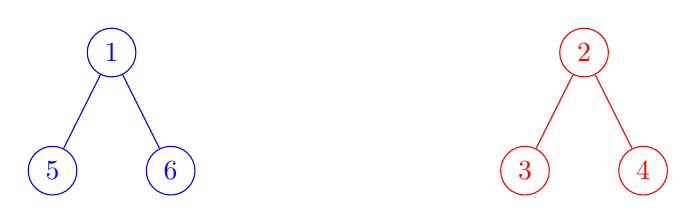
\begin{tikzpicture}
[
    edge from parent/.style={thick}
]
    \begin{scope}[edge from parent/.style={draw=blue}]
        \node [draw, circle, blue] {1}
            child {node [draw, circle, blue] {5}}
            child {node [draw, circle, blue] {6}};
    \end{scope}
    
    \begin{scope}[edge from parent/.style={draw=red}]
        \node [draw, circle, red] at (6, 0) {2}
            child {node [draw, circle, red] {3}}
            child {node [draw, circle, red] {4}};
    \end{scope}
\end{tikzpicture}
\end{center}

\end{frame}

\begin{frame}
\frametitle{Amogus Trick}

\begin{block}{Definition: Weight}
  w[i] := Number of Imposters in the subtree of $i$
\end{block}

Initially,

\begin{itemize}
  \item w[i] = 0, for $i \le n$
  \item w[i] = 1, for $i > n$
\end{itemize}

When we unite two vertices, we need to update the weight:
\begin{itemize}
  \item w[A] = w[A] + w[B]
\end{itemize}

\medskip

Such that: The answer is $\max\{w[i], w[i + n]\}$ for some $i$ which is root of the tree.

\end{frame}